\section*{Long-run of RNN-MSNN}

Test report

by E. Marquer, 2018/06/13 Synalp and Université de Lorraine

\subsection{Abstract}

The test is composed of 2 successive runs:
\begin{itemize}
\item id 1582586: batch-size 1, bptt 200 on grele-4;
\item id 1582587: batch-size 2, bptt 100 on grimani-6.
\end{itemize}

Run time is about 10h in each case, corresponding to 2h30 for an epoch.
In both case corpus batches rotation over epochs was disabled.

\subsubsection{Shared parameters}

\begin{longtable}[]{@{}ll@{}}
\hline
parameter & value\tabularnewline
\hline
\endhead
corpus & enwik8reduced\tabularnewline
history\_strategy & layer-constant-length\tabularnewline
max\_history & 25\tabularnewline
bptt & \emph{variable}\tabularnewline
batch\_size & \emph{variable}\tabularnewline
epochs & 4\tabularnewline
lr & 1e-3\tabularnewline
weight\_decay & 1.2e-6\tabularnewline
epochs & 4\tabularnewline
valid\_len & 500,000\tabularnewline
log\_interval & 500\tabularnewline
save\_interval & 500\tabularnewline
memory\_interval & 100\tabularnewline
hidden\_size & 460\tabularnewline
embed\_size & 400\tabularnewline
growth\_factor & 5\tabularnewline
rnn\_type & RNN\tabularnewline
reset\_hidden & False\tabularnewline
reset\_growth & True\tabularnewline
cuda\_on & True\tabularnewline
\hline
\end{longtable}

\subsection{Results}

At the end of each epoch, we see a spike in BPC, due to the first
evaluation of the epoch. As corpus rotation is disabled, it is not
surprising that with two batches over-fitting appears.

Moreover, we can note that run time is constant and memory usage tend to
a constant value (1.6 GiB), with no difference between 1 and 2 batches.
Note: the product \lstinline!bptt * batch_size! is equal for 1 and 2
batches, so this result is the one predicted by the equations.

\begin{figure}[h]
\centering
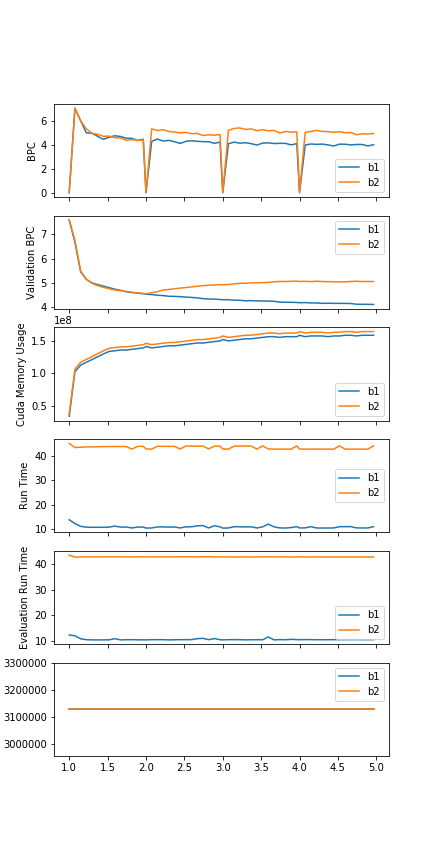
\includegraphics{parts/appendix/reports-gmsnn/docs_esteban-latex/test_reports/2018-06-13/batch_1_2_frac.png}
\caption{RAM third run}
\end{figure}

\begin{figure}[h]
\centering
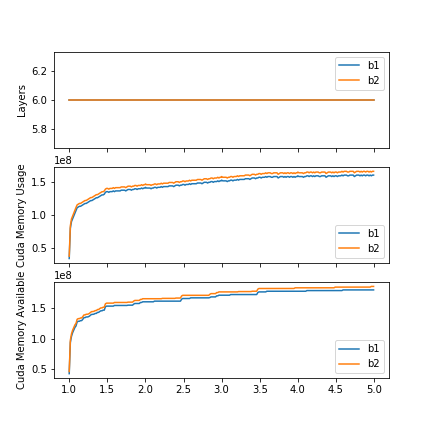
\includegraphics{parts/appendix/reports-gmsnn/docs_esteban-latex/test_reports/2018-06-13/batch_1_2_memory.png}
\caption{Memory usage}
\end{figure}

\subsection{Next steps}

\begin{itemize}
\item
  batches:

  \begin{enumerate}
  \def\labelenumi{\arabic{enumi}.}
  \item
    Implement corpus rotation
  \item
    See if corpus rotation solves over-fitting
  \item
    Compare run time on comparable machines
  \end{enumerate}
\item
  long run:

  \begin{enumerate}
  \def\labelenumi{\arabic{enumi}.}
  \item
    Continue batch 1 for more epochs
  \item
    See when over-fitting appears
  \end{enumerate}
\end{itemize}
